%auto-ignore
To evaluate the \isaffold against conventional Born-Mayer and/or Lennard-Jones models, we compare the
ability of each resulting short-range force field to reproduce benchmark ab
initio intermolecular interaction energies for a collection of representative
dimers. Such a metric is directly relevant for ab initio force field
development. Even for an empirically-parameterized force field, however,
fidelity to an accurate ab initio potential should be well correlated with the
highest level of accuracy and transferability achievable with a given
short-range methodology. 

We have developed the \isaffold, Born-Mayer, and Lennard-Jones force fields using 
benchmark energies calculated using the symmetry-adapted perturbation theory
based on density-functional theory (DFT-SAPT or SAPT(DFT) 
\cite{Misquitta2002,Misquitta2003,Misquitta2005,Heßelmann2005a,Podeszwa2006a,Heßelmann2002,Heßelmann2003,Heßelmann2002a,Jansen2001}).
DFT-SAPT provides interaction energies that are comparable in accuracy to 
those from CCSD(T) and which are rigorously free from basis set superposition error.
\cite{Podeszwa2005a,Riley2010}
Additionally, at second-order, DFT-SAPT also provides an explicit interaction
energy decomposition into physically-meaningful contributions: 
the electrostatic, exchange-repulsion, induction, and dispersion energies.
This decomposition is vital to the development of models as it allows the
development of separate terms for each type of short-range interaction. 
Terms of third and higher order are estimated using the \dhf correction 
\cite{Jeziorska1987} which contains mainly higher-order induction contributions.
Following prior work,\cite{Yu2011,McDaniel2013} and for the purposes of
fitting to the DFT-SAPT data, we keep the second-order induction term and the
\dhf term separate.
%

Since the Slater-ISA and Born-Mayer force fields describe only short-range interactions (i.e. those terms which are modulated by
the overlap of the monomer electron densities), they must both be supplemented with additional long-range
terms that describe the electrostatic, polarization, and dispersion
interactions. Here we have chosen a long-range potential of the form 
%
\begin{align}
\label{eq:isotropic-elr}
\vlr &= V_{\text{multipole}} + V_{\text{dispersion}} + \vdrude \\
\intertext{where}
V_{\text{multipole}} &= \sum \limits_{ij} \vmultipole
\intertext{includes distributed multipole contributions from each atom up to
quadrupoles,} 
V_{\text{dispersion}} &= - \sum\limits_{ij}\sum\limits_{n=3}^{6} \frac{C_{ij,2n}}{r_{ij}^{2n}} 
\label{eq:isotropic-dispersion}
\end{align}
describes isotropic dispersion, and 
\vdrude is the polarization energy modeled by Drude oscillators 
\cite{drude1902theory, Lamoureux2003}
as in
\citen{McDaniel2013}.
%
The accuracy of each of these terms is expected to minimize errors in the
long-range potential, simplifying the comparison between short-range force field functional forms.
Nonetheless, we expect that our results will be qualitatively insensitive to
the particular choice of long-range force field and acknowledge that simpler alternatives may
be preferred for the development of highly efficient simulation potentials.
In the case of the Lennard-Jones force field, we replace \cref{eq:isotropic-dispersion} with
the simple $C_{ij,6}/r_{ij}^{6}$ dispersion term that is standard to the
Lennard-Jones model. 

We used a test set consisting of one atom (argon) and 
12 small organic molecules (see \cref{fig:isotropic-molecules}) from which dimer
potentials could be generated (we will use the term `dimer' to mean two,
potentially dissimilar, interacting molecules or atoms), 
yielding 91 dimer combinations (13 homo-monomeric, 78 hetero-monomeric).
This wide range of systems allowed us to evaluate both the accuracy and
transferability of the Slater-ISA model compared to conventional Born-Mayer
and/or Lennard-Jones models.

    %%%%%%%%% 91 Dimer Test Set %%%%%%%%%%%%%
    \begin{figure}
      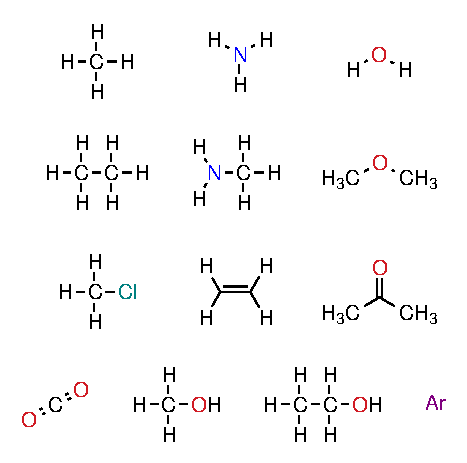
\includegraphics[width=0.6\textwidth]{isotropic/91_dimer_test_set.eps}
      \caption{
        The 13 small molecules included in the 91 dimer (13 homomonomeric, 78
        heteromonomeric) test set. Cartesian geometries for all of these
        molecules are given in \cref{sec:appendices-monomers}.
              }
      \label{fig:isotropic-molecules}
    \end{figure}
    %%%%%%%%% 91 Dimer Test Set %%%%%%%%%%%%%

A detailed description of this overall methodology is provided below.

\begin{subsection}{Construction of the 91 dimer test set}

Monomer geometries for each of the 13 small molecules were taken from the
experimental NIST
\mbox[CCCBDB] database\cite{Johnson2015NIST} and can be found in
\cref{sec:appendices-monomers}.
For acetone and methyl amine, experimental geometries were
unavailable, and thus
the computational NIST \mbox[CCCBDB] database was used to obtain geometries at
a high level of theory (B3LYP/\avtz for acetone, CCSD(T)/6-311G* for methyl
amine).
For each of the 91 dimers, a training set was constructed
using \saptpbeo interaction energies calculated at 1000 quasi-random dimer
configurations. These configurations were generated using Shoemake's
algorithm,\cite{Shoemake1992} subject to the constraint that the nearest atom pairs
be separated by between 0.75 and 1.3 of the sum of their van der Waals radii. 
This ensured adequate sampling of the potential 
energy surface in the region of the repulsive wall.
The DFT-SAPT interaction energies were evaluated using an asymptotically corrected
PBE0 functional (PBE0/AC) with monomer vertical (first) ionization potentials
computed using the $\Delta$-DFT approach at a PBE0/\avtz level of theory.
Unless otherwise noted, all DFT-SAPT calculations used an \avtz basis set in the 
dimer-centered form with midbond functions (the so-called DC+ form),
and were performed using the MOLPRO2009 software suite.\cite{MOLPRO-WIREs}
The midbond set consisted of a 5s3p1d1f even-tempered basis set with ratios
of 2.5 and centered at $\zeta = 0.5, 0.5, 0.3, 0.3$ for the s,p,d, and f shells,
respectively. This set was placed near the midpoint of the centers of mass of
the two interacting monomers.

A small fraction of DFT-SAPT calculations exhibited unphysical
energies, which were attributed to errors in generating the optimized
effective potential used during the \saptpbeo calculations; these points were
removed from the test set.

\end{subsection}
\begin{subsection}{\bsisa Calculations}


\bsisa atomic densities were obtained using CamCASP 5.8
\cite{camcasp5.8, WCMS:WCMS1172, orient4.8}
following the procedure of \citeauthor{Misquitta2014}\cite{Misquitta2014}
For the \bsisa calculations, an auxiliary basis was constructed from an RI-MP2
\avtz basis set with $s$-functions replaced by the ISA-set2
supplied with the CamCASP program;
CamCASP's ISA-set2 basis was also used for the ISA basis
set.\cite{Misquitta2014} A custom ISA basis set for Ar was used 
(even tempered, $n_{min} = -2, n_{max} = 8$)
\cite{Misquitta2014} 
as no published basis was available.
\bsisa calculations were performed with the A+DF algorithm, which allows the 
ISA functional to be mixed with some fraction, $\zeta$, of the density-fitting functional.
Following the recommendations of \citeauthor{Misquitta2014}\cite{Misquitta2014},
we have used $\zeta=0.1$ for the multipole moment calculations, 
and $\zeta=0.9$ for the density partitioning used to determine the \B coefficients. 


\end{subsection}
\begin{subsection}{Determination of $\Bisa{i}$}


The \bsisa-derived atomic exponents, $\Bisa{i}$, were obtained from a weighted
least-squares fit to the spherically averaged \bsisa atomic densities (shape functions),
$w_i(\mathbf{r})$.
In some cases, numerical instabilities and basis-set limitations of the \bsisa procedure
yielded densities that exhibited non-exponential asymptotic behavior.\cite{Misquitta2014}
To correct for these unphysical densities, we extrapolated the exponential decay
of the valence region to describe the \bsisa tails also. 
Details of this procedure can be found in
\cref{sec:workflow-exponent_algorithm}.
The ISA atom-in-molecule exponents were then derived via a log-weighted fit to
the tail-corrected shape-functions $w^a(\mathbf{r})$ for densities within the cutoff
$10^{-2} > w^a > 10^{-20}$ a.u.  This region was chosen to
reproduce the charge density most accurately in the valence regimes most likely to be relevant to
intermolecular interactions.


\end{subsection}
\begin{subsection}{Force Field Functional Forms and Parameterization}
    \label{sec:isotropic-FF-forms}

The general structure of the force fields \vtot for both the \isaffold and the 
Born-Mayer-type models are given by the following equations:

\begin{align}
%
\begin{split}
\label{eq:isotropic-bothff}
\vtot &= \sum\limits_{ij} \vrep_{ij} + \velst_{ij} + \vind_{ij} + \vdhf_{ij} +
\vdisp_{ij} \\[10pt]
\vrep_{ij} &= \Aex{ij} P(B_{ij}, r_{ij}) \exp(-B_{ij}r_{ij}) \\
\velst_{ij} &= -\Ael{ij} P(B_{ij}, r_{ij}) \exp(-B_{ij}r_{ij}) + \vmultipole \\
\vind_{ij} &= -\Aind{ij} P(B_{ij}, r_{ij}) \exp(-B_{ij}r_{ij}) + \vdrudeind \\
\vdhf_{ij} &= -\Adhf{ij} P(B_{ij}, r_{ij}) \exp(-B_{ij}r_{ij}) +
\vdrudescf \\
\vdisp_{ij} &= - \sum\limits_{n=3}^{6} f_{2n}(x) \frac{C_{ij,2n}}{r_{ij}^{2n}} \\
\A &= A_iA_j \\
\C &= \sqrt{C_{i,n}C_{j,n}} \\
f_{2n}(x) &= 1 - e^{-x} \sum \limits_{k=0}^{2n} \frac{(x)^k}{k!} \\
\end{split}
%
\intertext{For the \isaffold:}
%
\begin{split}
\label{eq:isotropic-isaff}
B_i &= \Bisa{i} \\
\B &= \sqrt{B_iB_j} \\
P(B_{ij},r_{ij}) &= \frac13 (B_{ij} r_{ij})^2 + B_{ij} r_{ij} + 1 \\
x &= B_{ij}r_{ij} - \frac{2 B_{ij}^2 r_{ij} + 3 B_{ij} }
{ B_{ij}^2 r_{ij}^2 + 3 B_{ij} r_{ij} + 3} r_{ij}
\end{split}
%
\intertext{For all Born-Mayer type models:}
%
\begin{split}
P(B_{ij},r_{ij}) &= 1 \\
x &= B_{ij}r_{ij}
\end{split}
%
\intertext{For the \saptff:}
%
\begin{split}
\label{eq:isotropic-saptff}
B_i &\equiv \Bip{i} = 2\sqrt{2I_i} \\
\B &= \frac{B_iB_j(B_i + B_j)}{B_i^2 + B_j^2}
\end{split}
%
\intertext{For the \bmsisaff:}
%
\begin{split}
    B_i &= 0.84\Bisa{i} \\
    \B &= \sqrt{B_iB_j}
\end{split}
%
\end{align}
%

Of the parameters in these force fields, only the coefficients $A_i$ were fit
to reproduce DFT-SAPT dimer energies (details below). All other force field
parameters were derived from first-principles atom or atom-in-molecule properties.
Exponents for the \isaffold and the \bmsisaff were derived from \bsisa calculations,
while exponents for the \saptff were determined from vertical ionization potentials
of the isolated atoms.
Dispersion coefficients (\C) were either used directly from \citen{McDaniel2013} or
were parameterized using analogous methods in the case of argon.
Distributed multipoles $Q_t^i$ for each system were obtained from the \bsisa-based
distributed multipoles scheme (ISA-DMA) \cite{Misquitta2014}, with the expansion
truncated to rank 2 (quadrupole). 
Note that here, $t=00,10,\dots,22s$ denotes the rank of the multipole in 
the compact notation of \citeboth{stone2013theory}.
% AJM : This is a bit confusing. Can you explain?
(In addition to rank 2 ISA-DMA multipoles, we also tested the use of DMA4
multipoles\cite{Stone2005} 
as well as the use of rank 0 charges obtained from the 
rank truncation or transformation\cite{Ferenczy1997} of either ISA-DMA or DMA4
multipoles; the effect of including a Tang-Toennies damping
factor\cite{McDaniel2013,Tang1984} was studied in all cases.
Each of these alternative long-range electrostatic models proved either
comparably or less accurate for both the \isaffold and the \saptff in terms of their
ability to reproduce the DFT-SAPT electrostatic energy, and are not discussed
further.)
Long-range polarization ($V_{shell}$) was modeled using Drude oscillators in a manner
identical to \citen{McDaniel2013}. As in our prior work, during parameterization,
the Drude energy was partitioned into 2\super{nd} (\vdrudeind) and 
higher order (\vdrudescf) contributions, where \vdrudeind is the Drude oscillator
energy due to static charges (excluding intra-molecular contributions), and
\vdrudescf is the difference between the fully converged Drude energy,
$V_{shell}$, and \vdrudeind.  Force field parameters for all homo-monomeric
systems are located in the \si of \citen{VanVleet2016}. 

A weighted least-squares fitting procedure was used to fit $A_i$
parameters to the benchmark \saptpbeo interaction energies on a 
component-by-component basis.
That is, four separate optimizations\cite{McDaniel2013}  were
performed to directly fit \vrep, \velst, \vind, and \vdhf to, respectively, the
following DFT-SAPT quantities (notation as in \citen{Heßelmann2005a}):
%
\begin{align}
\begin{split}
\erep &\equiv E^{(1)}_{\text{exch}} \\
\eelst &\equiv E^{(1)}_{\text{pol}} \\
\eind &\equiv E^{(2)}_{\text{ind}} + E^{(2)}_{\text{ind-exch}} \\
\edhf &\equiv \delta(\text{HF}).
\end{split}
%
\intertext{
For \vdisp, no parameters were directly fit to the DFT-SAPT dispersion,
}
%
\edisp &\equiv E^{(2)}_{\text{disp}} + E^{(2)}_{\text{disp-exch}},
\end{align}
%
but were instead obtained solely from monomer properties as described above.
Finally, note that no parameters were directly fit to the total DFT-SAPT
energy,
%
\begin{align}
\etot = \erep + \eelst + \eind + \edhf + \edisp,
\end{align}
%
for either the \isaffold or the \saptff. Rather, \vtot was calculated according to \cref{eq:isotropic-bothff}.

Data points for each fit were weighted using a Fermi-Dirac functional form
given by
%
\begin{align}
\label{eq:isotropic-weighting-function}
w_i = \frac{1}{\exp((-E_i - \mu_{\text{eff}})/kT) + 1},
\end{align}
%
where $E_i$ is the reference energy and $\mu_{\text{eff}}$ and $kT$ were treated as
adjustable parameters. The parameter $kT$, which sets the energy scale for the
weighting function, was taken to be $kT = \lambda |E_{\text{min}}|$; here $E_{\text{min}}$
is an estimate of the global minimum well depth. Unless otherwise stated, we have used
$\lambda = 2.0$ and $\mu_{\text{eff}} = 0.0$.   
These defaults were chosen to minimize overall average attractive RMSE for all 91 dimer
sets. 
Increases or decreases in the $\lambda$ factor correspond to the weighting of
more or fewer repulsive configurations, respectively.  

In the case of Lennard-Jones, the standard Lennard-Jones functional form was
used for the van der Waals terms, with Coulomb and polarization terms modeled
exactly as for the \isaffold:
\begin{align}
%
\vtot^{\text{LJ}} &= \sum\limits_{ij} \frac{A_{ij}}{r^{12}_{ij}} - \frac{C_{ij,6}}{r^{6}_{ij}} + \vdrude + \vmultipole
%
\end{align}
%
Lorentz-Berthelot combination rules were used to obtain heteroatomic $A_{ij}$
and $C_{ij}$ parameters. Unlike with the \isaffold and Born-Mayer models, $\vtot^{\text{LJ}}$ was fit to
the total \saptpbeo energy, with $A_{ij}$ and $C_{ij,6}$ as fitting parameters. The
weighting function from \cref{eq:isotropic-weighting-function} was used in fitting.

%% In order to also compare the \isaffold to simple non-polarizable Lennard-Jones force
%% fields, we also parameterized a version of $\vtot^{\text{LJ}}$ using only rank 0 charges and
%% $\vdrude = 0$; these results are shown in the Supporting Information.

\end{subsection}
\begin{subsection}{Potential Energy Surface Scans}


In order to visually assess fit quality, representative one-dimensional scans
of the potential energy surface were calculated for several dimer pairs along
low-energy dimer orientations. For each dimer pair, the minimum energy
configuration of the 1000 random dimer points was selected as a starting
configuration, and additional dimer configurations (not necessarily included in the
original 1000 points) were generated by scanning along some bond vector. In the case of the
ethane dimer, two carbon atoms (one on each monomer) were used; for acetone,
the carbonyl carbon on each monomer defined the bond vector.


\end{subsection}


\begin{subsection}{Molecular Simulations}

All bulk simulations were run using OpenMM release version 7.0.
\cite{Eastman2013}
Enthalpies of vaporization were computed from 
%
\begin{align*}
\Delta H_{\text{vap}} = (E_{\text{pot}}(g) + RT) - E_{\text{pot}}(l)
\end{align*}
%
where $E_{\text{pot}}(g)$ and $E_{\text{pot}}(l)$ were determined from NVT
simulations at the experimental gas and liquid densities, respectively.
Calculated liquid
densities were determined from NPT simulations. In all cases, the OPLS/AA
force field was used for the intramolecular potential.
\cite{Jorgensen1996}
All simulations used a Langevin integrator with a 0.5 fs time step and a 1
ps$^{-1}$ friction coefficient; NPT simulations used a Monte Carlo barostat
with a trial volume step every 5\super{th} move. Periodic boundary conditions,
particle-mesh Ewald, and a non-bonding cutoff of 1.2nm with added long-range
corrections were used to simulate a
unit cell of 222 molecules. After an equilibration period
of at least 600ps, simulation data was gathered from production runs lasting
at least 200ns. 



\end{subsection}
